
\section{Related work}\label{sec:embedsom_relwork}

% In this work, we specifically reflect the needs of many areas of life sciences where large multidimensional point-cloud-like datasets occur, such as population biology, microscopy imaging, metagenomics, and others.

% Single-cell cytometry~\cite{adan2017flow} forms a canonical example of this niche: The recent development of hardware and measuring equipment has enabled a precise collection of multiple features of each of millions of cells in a sample. Clinicians and biologists commonly measure metrics such as protein expression on the cell surface using antibody-based markers. For instance, the marker detection may be performed optically by exciting fluorochromes with a laser and measuring emission spectra or using a specific binding of heavy metal ions detected by mass spectrometry techniques such as time-of-flight~\cite{spitzer2016mass}. Both methods allow cheap acquisition of data about more than 50 selected features at once, typically with several million single-cell measurements from each sample~\cite{vanikova2021omip,rodriguez2020systems}. Additionally, the development of single-cell sequencing methods has enabled to sequence the mRNA present in the individual cells~\cite{ziegenhain2017comparative}, typically yielding a dataset with thousands of data points of dimensions higher than $10^4$.

% Due to the variability in the samples, data, and measurements, analyzing and interpreting the results is challenging. Biologists usually analyze the datasets by linearly projecting the features to 2-dimensional plots and manually selecting the cells of interest in a process called gating~\cite{bashashati2009survey}. While computationally simple and easily interpretable by humans, gating gets extremely error-prone as the dimensionality of the dataset increases. It does not provide good support for detecting dataset features of dimensionality higher than $2$, such as complicated pathways and loops in cell phenotypes. Similarly, applying algorithms for clustering analysis provided good detection of cell phenotype clusters but minimal reliability in pathway-style feature detection~\cite{saelens2018comparison}.

% \begin{figure}
% \centering
% {\linewidth=21pc
% \begin{tikzpicture}[font=\tiny\sffamily\bfseries, inner sep=1pt]
% \node[inner sep=0, anchor=south west] (img) at (0,0) {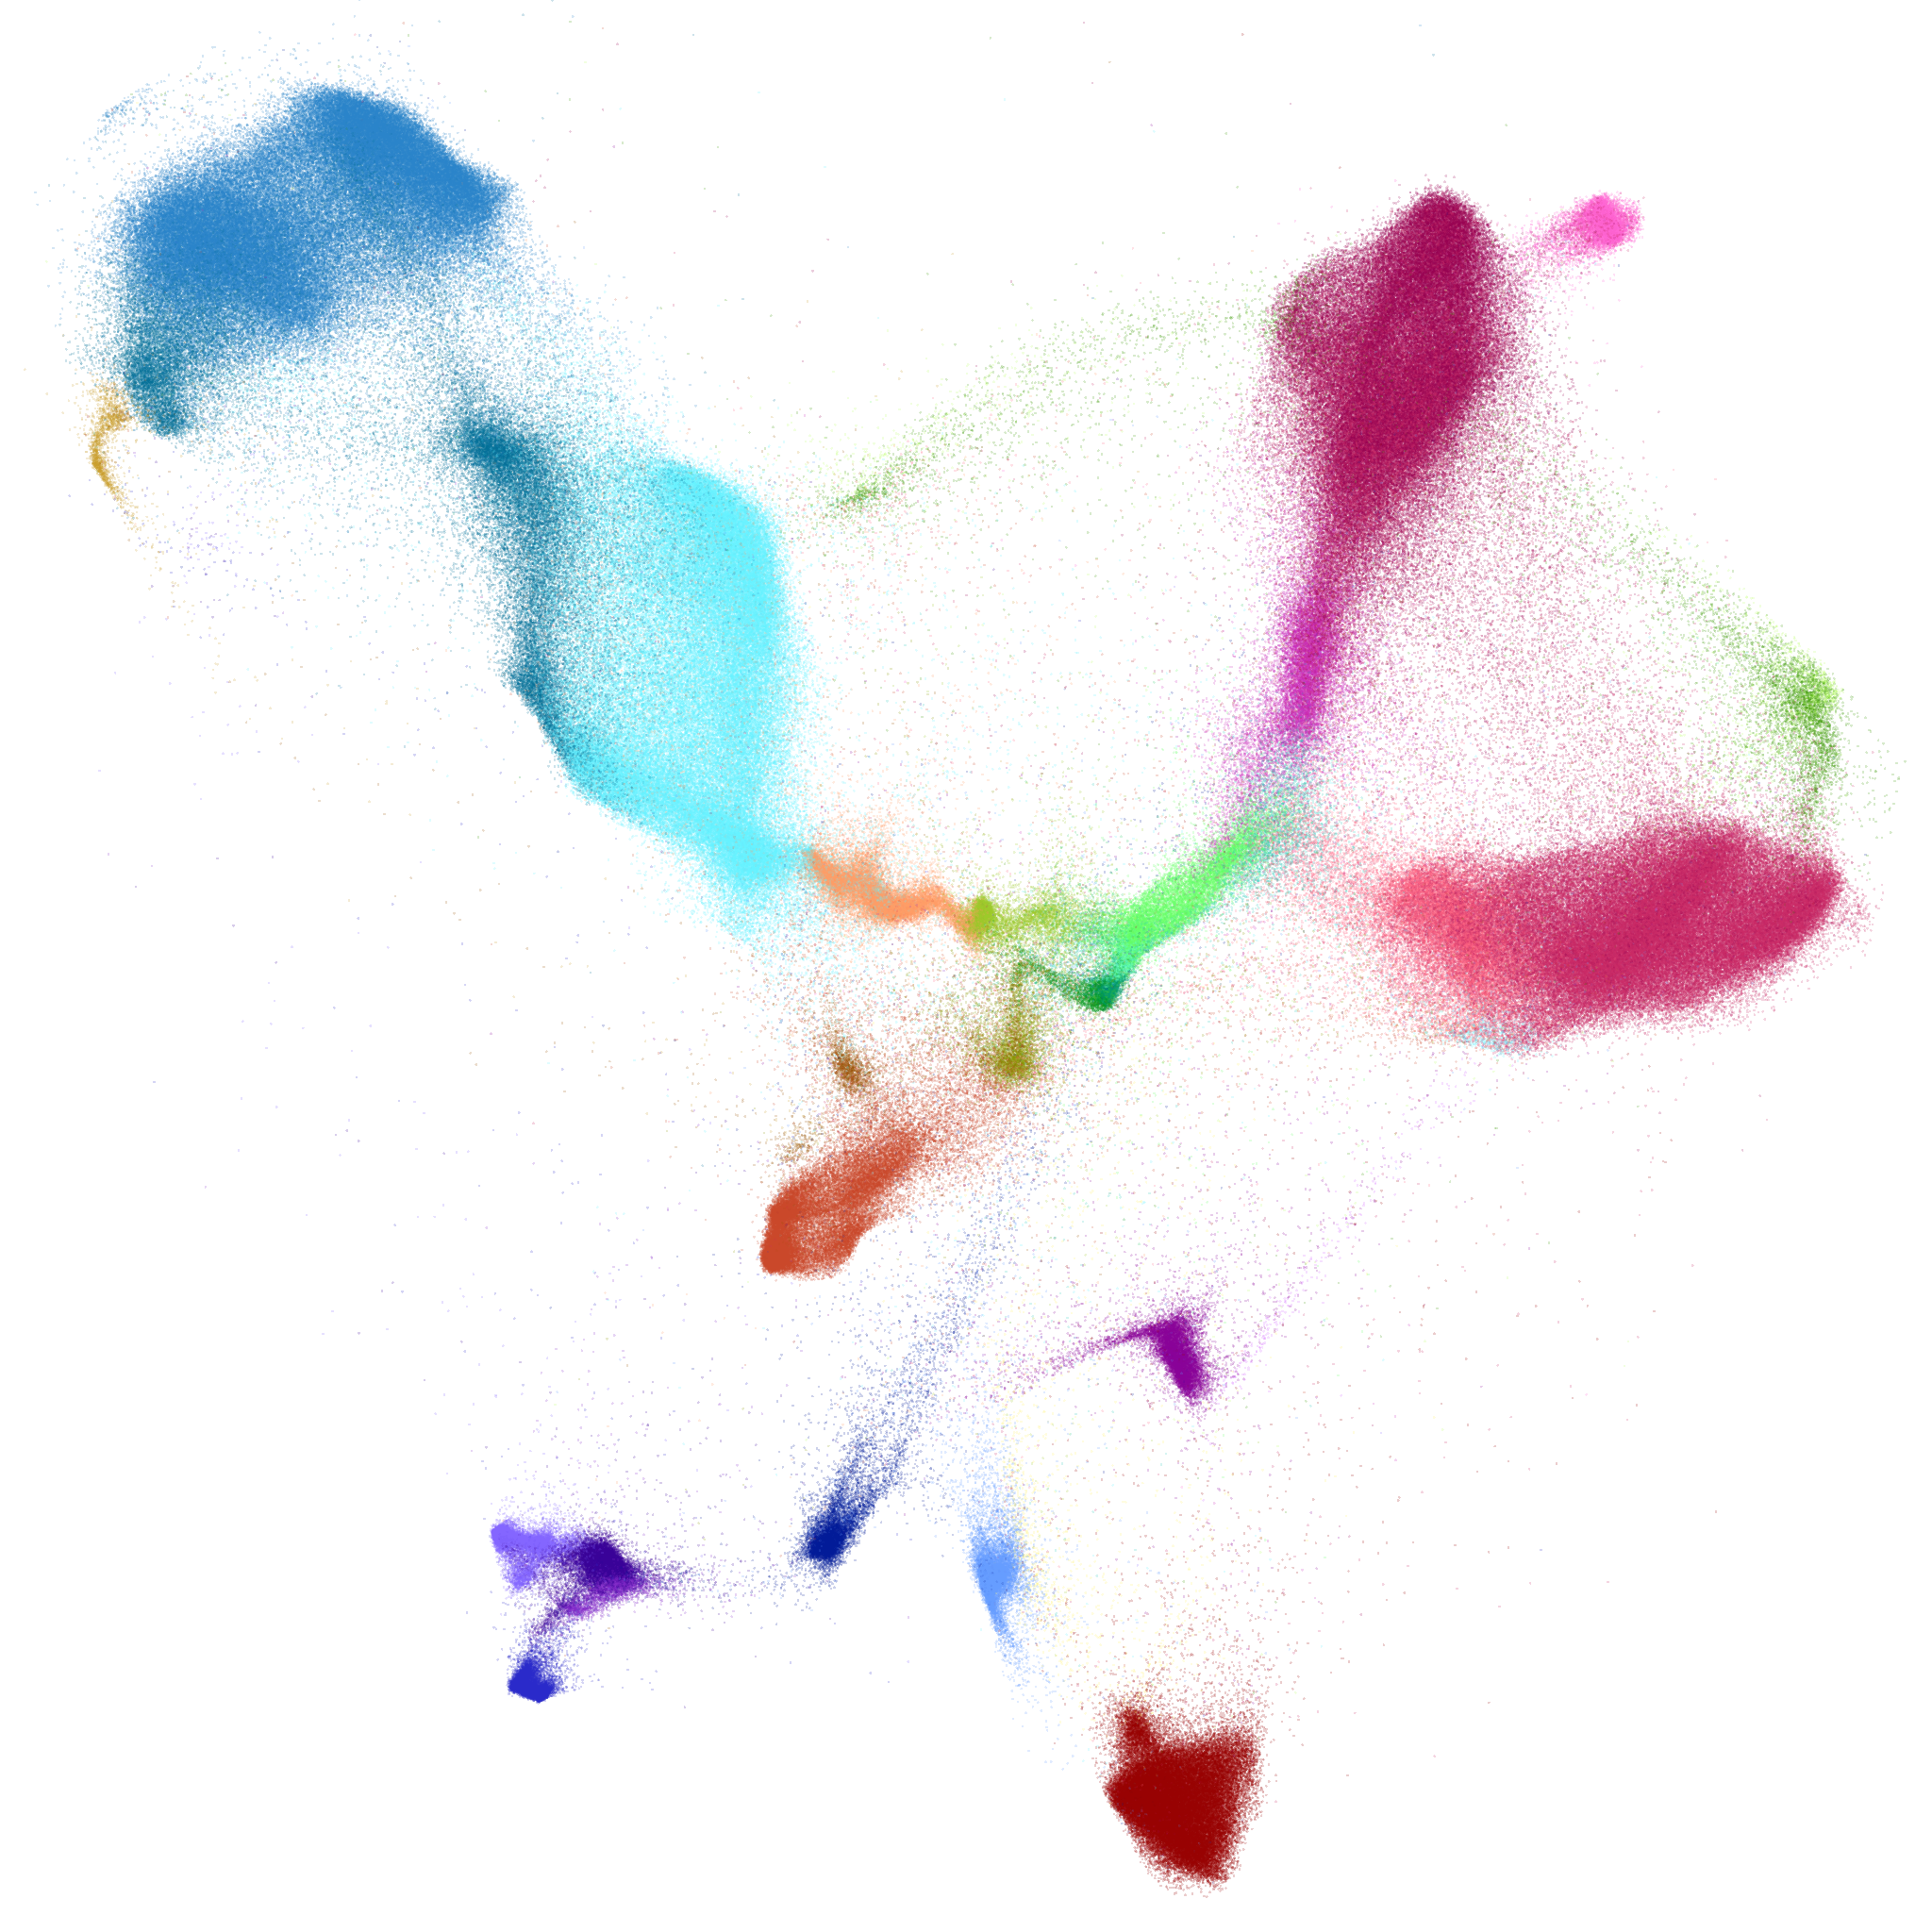
\includegraphics[width=\linewidth]{embedsom/pic/samusik-embedsom.png}};
% %\draw[help lines, xstep=0.1\linewidth, ystep=0.1\linewidth] (img.south west) grid (img.north east);
% \node[circle, draw] (A) at (0.5\linewidth,0.9\linewidth) {A};
% \node[circle, draw] (B) at (0.8\linewidth,0.2\linewidth) {B};
% \node[circle, draw] (C) at (0.2\linewidth,0.4\linewidth) {C};
% \node[circle, draw] (D) at (0.5\linewidth,0.266\linewidth) {D};
% \draw (A) to (0.45\linewidth,0.75\linewidth);
% \draw (A) to (0.9\linewidth,0.666\linewidth);
% \draw (B) to (0.55\linewidth,0.2\linewidth);
% \draw (B) to (0.65\linewidth,0.125\linewidth);
% \draw (B) to (0.55\linewidth,0.45\linewidth);
% \draw (C) to (0.5\linewidth,0.5\linewidth);
% \draw (C) to (0.275\linewidth,0.225\linewidth);
% \end{tikzpicture}}
% \caption{
% Example EmbedSOM projection of $841,644$ data points with $39$-dimensional single-cell measurements, representing the immune cell contents of bone marrow~\cite{samusik2016automated}. Colors were assigned manually to differentiate biologically relevant cell populations. Manual intervention in the unsupervised dimensionality reduction process would allow the user to fix several visualization deficiencies: overlapping pathways (labeled with~A), disconnected pathways (B), display of features in the small complex cell clusters (C), and the orientation and positioning of clusters that were chosen arbitrarily by the reduction process, not reflecting any biologically relevant features (D).
% }
% \label{fig:samusik}
% \end{figure}

% The development of non-linear dimensionality reduction algorithms in the last two decades has resolved many challenges. The new visualization-oriented methods, represented in the field mainly by t-SNE~\cite{maaten2008visualizing}, provided output that was sufficiently intuitive to understand, yet gave a satisfactory view of the highly complicated features that can not be observed by gating and projections. The tremendous success was quickly followed by new alternative algorithms that optimize different aspects of the process. UMAP~\cite{becht2019dimensionality} is currently a common choice for both visualization and a starting point of analysis, followed by PHATE~\cite{moon2019visualizing}, scvis\cite{ding2018interpretable}, TriMap\cite{amid2019trimap}, and others. For illustration, a typical example visualization is provided in~Figure~\ref{fig:samusik}, along with the description of common visualization problems.

% Following the plethora of newly introduced algorithms, a discussion unfolded to assess the optimality of the obtained visualization. Reviews have focused not only on reproducibility and robustness (i.e., susceptibility to significant changes in output caused by minor variations in data or different random seeds) but also on the representation of biologically valid features. Vast resources were invested into modifying the algorithms, especially t-SNE, to maximize various metrics, including convergence speed~\cite{belkina2019automated}, general performance~\cite{linderman2019fast}, robustness~\cite{polivcar2021embedding}, and the (very informally specified) quality of the display of local and global relations in data~\cite{kobak2019heavy,kobak2021initialization}. Some features required for high visualization quality are showcased in~Figure~\ref{fig:samusik}.

% User interaction possibilities in the dimensionality reduction process were therefore largely neglected, except for prohibitively small datasets where the use of force-based graph layouts and similar algorithms did not pose a throughput challenge. As one of few exceptions, van~Unen~et~al.~\cite{unen2017visual} and Chatzimparmpas~et~al.~\cite{chatzimparmpas2020t} achieved a methodological advance by extending the t-SNE algorithm, producing HSNE and t-viSNE respectively. HSNE organizes and visualizes a small data model dynamically using t-SNE, providing an intuitive way for the user to zoom into various compartments of the dataset, following a hierarchical structure of clusters. t-viSNE focuses on interactive use of t-SNE for exploration of complex dataset properties, but only of relatively small datasets.

% Compared to HSNE, our developments in BlosSOM provide two significant improvements: Full dataset may be rendered at all times (giving an unprecedented high-definition view of the features), which is enabled by a more efficient design of the base algorithm. Additionally, no hierarchical structure or no fixed layouting algorithm is imposed on the user, improving the display of structures that are hard to visualize or capture with hierarchical methods, such as the inter-cluster pathways.


% \subsection{GPU acceleration}

The essential component of our success is GPU acceleration of the projection computation which needs to be fast enough to re-calculate the embedding in real-time. 
In the following, we address the most relevant works that influenced or inspired our solution.

% One of the first GPU-accelerated dimensionality reduction methods was proposed in the work of Yeh et al.~\cite{yeh2010efficient} about twelve years ago. The first part uses $k$NN search with $k$-$d$-tree indexing structure. The GPU was used to compute Euclidean distances and to construct the tree using the radix sort algorithm. The projection itself used the Krylov subspace method for local linear embedding (LLE), which can be realized as a sparse matrix-vector multiplication so it was computed by cuBLAS. Despite the limited properties of the GPUs of the time, they were able to achieve $30$--$60\times$ speedup to the CPU implementation.

% A slightly different approach takes methods based on \emph{Principal Component Analysis} (PCA) algorithm. These methods are quite popular mainly since the principal components can be computed as eigenvectors of the data covariance matrix; thus, it can be implemented using linear algebra libraries. Martel et al.~\cite{martel2018implementation} proposed the implementation of PCA for CUDA and FPGAs. They have used the Jacobi method for the eigenvector decomposition, and the implementation heavily relied on Thrust and cuBLAS libraries. PCA is also used in more elaborate projection methods such as \emph{secant-based dimensionality reduction}~\cite{kvinge2018gpu}. The PCA is used to initialize a projection matrix, which is subsequently iteratively improved by a \emph{secant set} --- a set of normalized differences of all input point pairs. The projection matrix is multiplied with every secant to find a \emph{secant projection} with minimal $L_2$ norm. Although this method is theoretically intriguing, the GPU implementation is quite straightforward, using simple kernels and the cuSolver library.

Being one of the most profound visualization methods, \emph{t-SNE} was studied to explore the possibilities of having a fast GPU-enabled implementation. One of the initial implementations was t-SNE-CUDA library~\cite{chan2018t}. The most complicated step (computing the attractive forces of the N-body simulation) is handled as a multiplication of a sparse matrix and a vector by the CUSparse library. This work was slightly improved a year later \cite{chan2019gpu} when the authors replaced the CUSparse library with their implementation of multiplication, which takes advantage of atomic operations to perform the reduction in scalar sums.

% t-SNE can be improved by applying a hierarchical approach which can help both with the stability of the results and the computational demands of the algorithm. One of the first representatives that used a hierarchical approach and GPU acceleration was the Anchor-t-SNE (AtSNE) algorithm~\cite{fu2019atsne} which uses anchor points, selected representatives of the data which are projected first, and the remaining points are projected based on their proximity to the anchor points. A similar idea is used in the Barnes-Hut approximation of t-SNE\cite{van2014accelerating} which constructs a tree data structure that helps compute repulsive forces. This method was used in the work of Meyer et al.~\cite{meyer2020improving}, who implemented a warp-optimized CUDA version SWW-tSNE. Unlike the original t-SNE-CUDA, they have decided to use cuBLAS for the computation of attractive forces. The SWW-tSNE was later improved and accompanied with SWW-AtSNE~\cite{meyer2022global}, a warp-optimized version of anchor-based implementation of t-SNE~\cite{fu2019atsne}.

Perhaps the most popular contemporary method for data visualization is the \emph{Uniform Manifold Approximation and Projection} algorithm (UMAP), which often produces better results than t-SNE at the cost of higher computational demands. There are two GPU implementations worth mentioning which were both made part of RAPIDS cuML library~\cite{tegegne2021parallel, nolet2020bringing}. They both use a similar approach, implementing a kNN approximation based on gradient descent methods. The first implementation~\cite{tegegne2021parallel} relies more on existing solutions and libraries, and the second one~\cite{nolet2020bringing} is slightly more low-level as they implement the embedding using custom kernels.

Even though the presented methods (especially t-SNE) exceeded the speedup of two orders of magnitude, they are still quite far from real-time processing when the number of points reaches the order of millions. The proposed EmbedSOM projection is based on SOMs and linear projection based on $k$NN search~\cite{kratochvil2019generalized,kratochvil2020shinysom}, which is technically closest to the work of Yeh et al.~\cite{yeh2010efficient}. For the SOM part, we have adapted the state-of-the-art implementation of $k$-means algorithm~\cite{krulis2020detailed} since SOM shares many of its steps. The crucial part of the projection is the $k$NN search, which is also repeated in the aforementioned papers; however, we have found that the solution based on bitonic-sorting~\cite{krulivs2015optimizing} performs the best in our case.

